%Группа 11-2 Модуль 3
\cheadbf{Модуль 3 Занятие 2}
\begin{listofex}
	\item
	\begin{minipage}[t]{0.67\textwidth}
		На рисунке изображен график функции \( f(x)=kx+b \). Найдите \( f(-9) \).
	\end{minipage}
	\begin{minipage}[c]{0.2\textwidth}
		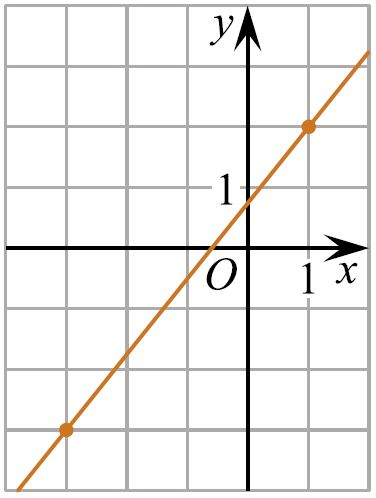
\includegraphics[align=t, width=0.8\textwidth]{pics/G112M3C2-1}
	\end{minipage}
	\item
	\begin{minipage}[t]{0.67\textwidth}
		На рисунке изображены графики двух линейных функций. Найдите абсциссу точки пересечения графиков.
	\end{minipage}
	\begin{minipage}[c]{0.2\textwidth}
		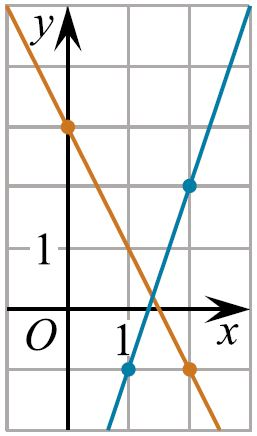
\includegraphics[align=t, width=0.8\textwidth]{pics/G112M3C2-2}
	\end{minipage}
	\item
	\begin{minipage}[t]{0.57\textwidth}
		На рисунке изображен график функции \( f(x)=\dfrac{x^2}{a}+bx+c \). Найдите \( f(3,5) \).
	\end{minipage}
	\begin{minipage}[c]{0.3\textwidth}
		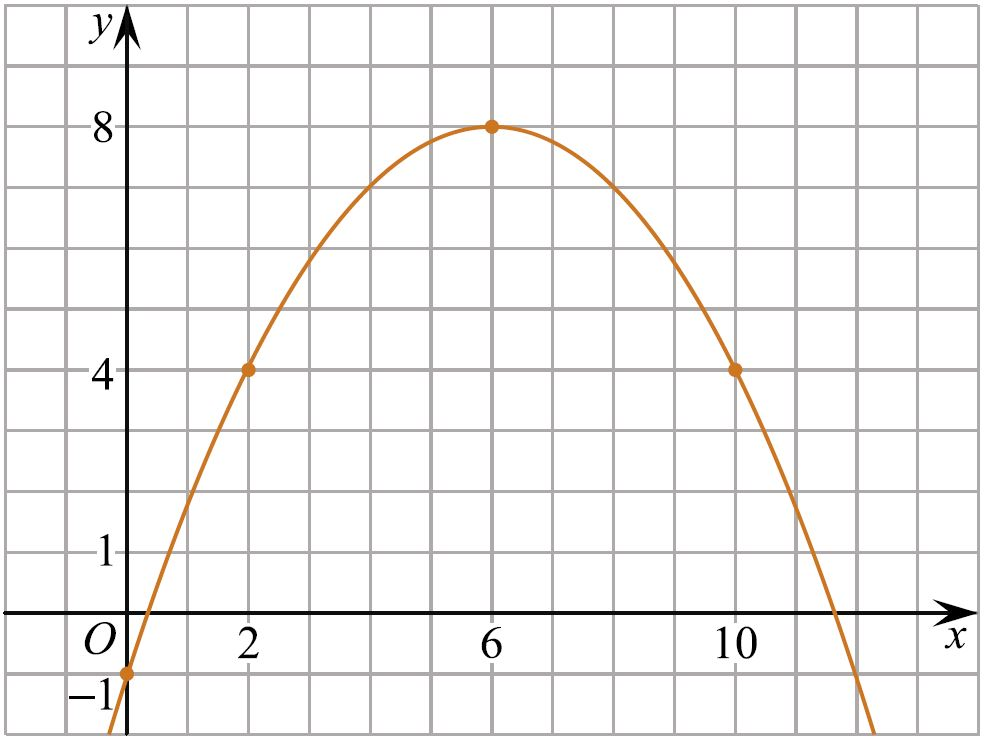
\includegraphics[align=t, width=\textwidth]{pics/G112M3C2-3}
	\end{minipage}
	\item
	\begin{minipage}[t]{0.57\textwidth}
		На рисунке изображен график функции \( f(x)=\dfrac{x^2}{a}+bx+c \). Найдите \( f(4) \).
	\end{minipage}
	\begin{minipage}[c]{0.3\textwidth}
		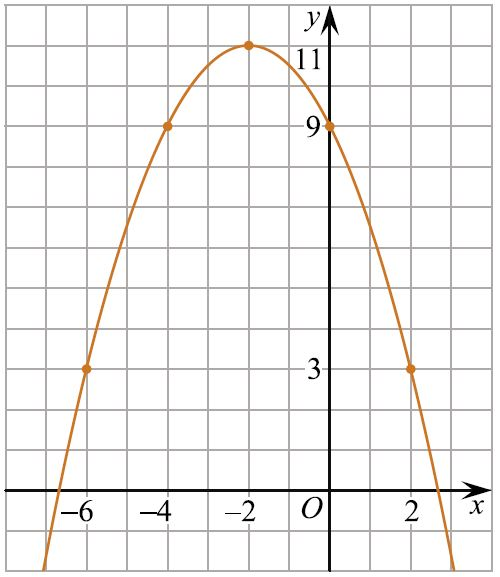
\includegraphics[align=t, width=\textwidth]{pics/G112M3C2-4}
	\end{minipage}
	\item
	\begin{minipage}[t]{0.57\textwidth}
		На рисунке изображен график функции \( f(x)=\dfrac{k}{x}+a \). Найдите, при каком значении \( x \) значение функции будет равно \( 0,8 \).
	\end{minipage}
	\begin{minipage}[c]{0.3\textwidth}
		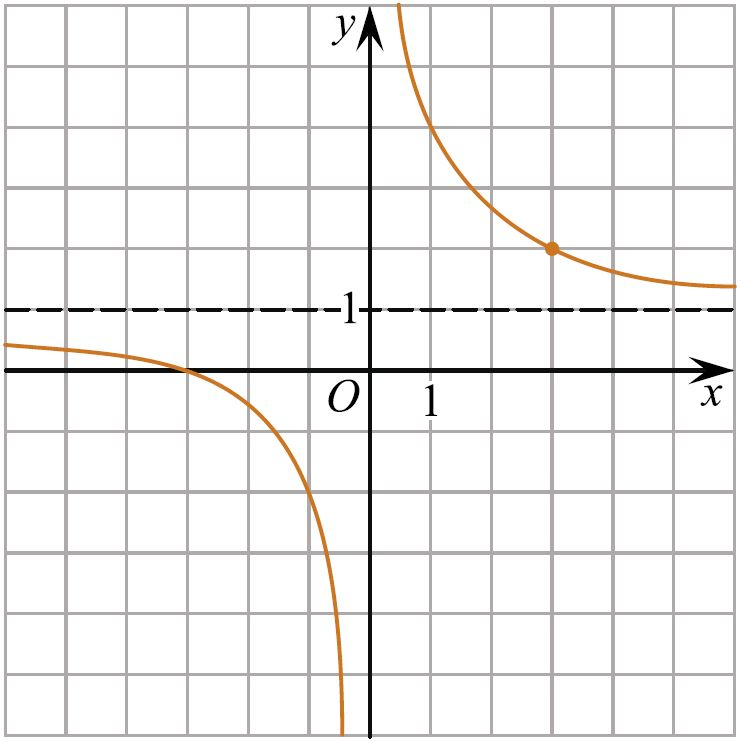
\includegraphics[align=t, width=\textwidth]{pics/G112M3C2-5}
	\end{minipage}
	\item
	\begin{minipage}[t]{0.57\textwidth}
		На рисунке изображены графики функций \( f(x)=2x^2+11x+11 \) и \( y=ax^2+bx+c \), которые пересекаются в точках \( A \) и \( B \). Найдите абсциссу точки \( B \).
	\end{minipage}
	\begin{minipage}[c]{0.3\textwidth}
		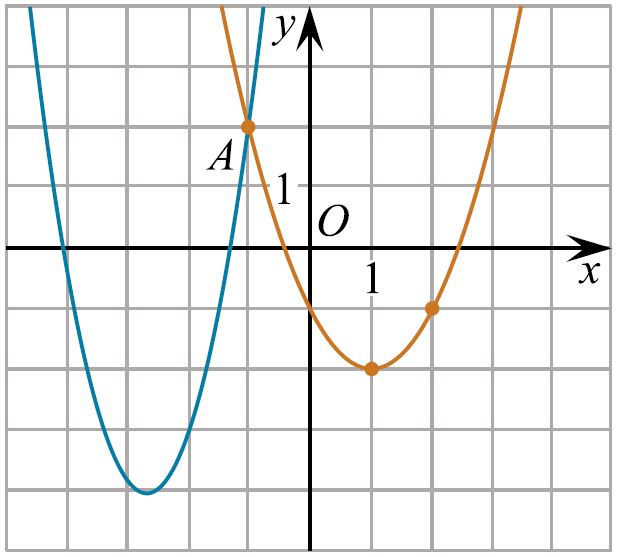
\includegraphics[align=t, width=\textwidth]{pics/G112M3C2-6}
	\end{minipage}
	\item Велосипедист выехал с постоянной скоростью из города \( A \) в город \( B \), расстояние между
	которыми равно \( 70 \) км. На следующий день он отправился обратно в \( A \) со скоростью на \( 3 \) км/ч больше прежней. По дороге он сделал остановку на \( 3 \) часа. В результате велосипедист затратил на обратный путь столько же времени, сколько на путь из \( A \) в \( B \). Найдите скорость велосипедиста на пути из \( B \) в \( A \). Ответ дайте в км/ч.
	\item В сосуд, содержащий \( 5 \) литров \( 12 \)--процентного водного раствора некоторого вещества,
	добавили \( 7 \) литров воды. Сколько процентов составляет концентрация получившегося раствора?
	\item При производстве в среднем на каждые \( 2982 \) исправных насоса приходится \( 18 \) неисправных.
	Найдите вероятность того, что случайно выбранный насос окажется неисправным.
\end{listofex}
%\newpage
%\title{Занятие №2}
%\begin{listofex}
%	
%\end{listofex}
%\newpage
%\title{Домашняя работа №1}
%\begin{listofex}
%	
%\end{listofex}
%\newpage
%\title{Занятие №3}
%\begin{listofex}
%	
%\end{listofex}
%\newpage
%\title{Занятие №4}
%\begin{listofex}
%	
%\end{listofex}
%\newpage
%\title{Домашняя работа №2}
%\begin{listofex}
%	
%\end{listofex}
%\newpage
%\title{Занятие №5}
%\begin{listofex}
%	
%\end{listofex}
%\newpage
%\title{Занятие №6}
%\begin{listofex}
%	
%\end{listofex}
%\newpage
%\title{Домашняя работа №3}
%\begin{listofex}
%	
%\end{listofex}
%\newpage
%\title{Подготовка к проверочной работе}
%\begin{listofex}
%	
%\end{listofex}
%\newpage
%\title{Проверочная работа}
%\title{Вариант 1}
%\begin{listofex}
%	
%\end{listofex}
%\newpage
%\title{Проверочная работа}
%\begin{listofex}
%	
%\end{listofex}